
\section{Transit detection methods in literature}
\label{sec:detection_lit}

The following subsections describe previously proposed methods for transit detection in further detail. The pipelines of the TESS and Kepler missions are included in the description, because they have a built-in module for transit detection. Classical methods are described first, after which we describe the more recent developments in AI in the task of transit detection.

\subsection{Box and Transit Least Squares}

The Box Least Squares (BLS) algorithm, proposed by \cite{kovacs2002box}, is widely adopted in the task of transit signal detection (e.g. \cite{kunimoto2020searching}, \cite{rizzuto2020tess}. Its simplified model of the transit signal makes it a relatively efficient algorithm, because the model is only parameterized by the transit depth, duration and timing of the signal. The model is fitted to the data by minimizing the squared error, or similarly, maximizing the log likelihood of the model with respect to the transit depth $\delta$ for a given configuration of orbital period $P$, transit duration $\tau$ and epoch $t_0$\footnote{\url{https://docs.astropy.org/en/stable/timeseries/bls.html}. Accessed: 18-08-2021.}. The log likelihood at different values for $P$, maximized over $\{\delta$, $\tau$, $t_0\}$ is proportional to the Signal Residue ($SR$) as defined by \cite{kovacs2002box}. The $SR$ at each given trial period can be used to define the BLS periodogram, i.e. $SR$ over $P$. More commonly, the Signal Detection Efficiency ($SDE$) is used instead of $SR$, which is defined as
\begin{equation}
    SDE = \frac{SR_{\text{peak}} - \textit{mean}\,(SR)} {\textit{std}\,(SR)},
\end{equation}
where $SR_{\text{peak}}$ is the maximum $SR$ in the periodogram, and $\textit{mean}\,(SR)$ and $\textit{std}\,(SR)$ are the mean and standard deviation of the periodogram respectively.

An example of the BLS periodogram is shown in Figure \ref{fig:bls_example}, in which we can see how the peaks in the periodogram can be used for detection. For example, a peak in the at a given period $P$ could indicate the detection of a signal with corresponding parameters $\{\delta$, $\tau$, $t_0$, $P\}$, which are provided for each point in the periodogram. However, as is clear from the figure, the harmonics of the signal may be confusing and lead to wrong detections.

\begin{figure}
    \centering
    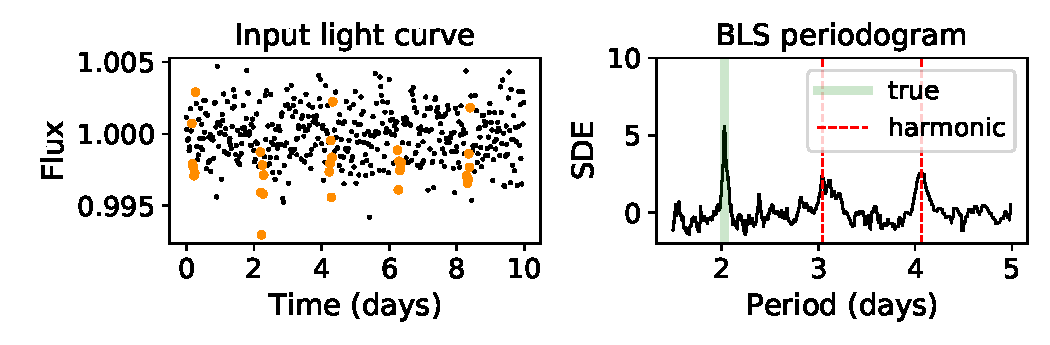
\includegraphics[width=0.6\linewidth]{Background/Figures/BLS_example.pdf}
    \caption{The BLS algorithm applied to the same light curve from Figure \ref{fig:folding}, with the transit signals visualized in orange. The highest peak in the periodogram corresponds to the correct period $P$ of the signal. However, the harmonics of the signal, e.g. $3/2P$ and $2P$ as shown here, also produce peaks.}
    \label{fig:bls_example}
\end{figure}

Instead of using the SDE to set a detection threshold, a detection threshold could be set on the signal-to-noise ratio (SNR) of transit candidates. Ignoring the presence of time-dependent noise, the SNR can be defined as $\delta / \sigma_w \cdot \sqrt{n_t}$ with $n_t \,\propto\, \tau$ the number of measurements that belong to the transit signal and $\sigma_w$ the estimated white noise in the detrended light curve. However, \cite{pont2006effect} show that a detection threshold for BLS can be set better if time-dependent noise is accounted for in the approximation of the SNR. This is likely because background patterns with time scales similar to the transit duration could remain intact after detrending.

Several variants to BLS exist. For example, \cite{carter2013quasiperiodic} relax the assumption of strictly periodic signals, and use a quasi-periodic transit model that is fitted to the data. \cite{foreman2016population} omit the periodicity assumption altogether and use an algorithm similar to BLS to search for monotransits. In their work, a box function is fitted to the data at multiple points in time, and a detection threshold for single events is set on the SNR above the noise floor determined by a sliding median filter.

More recently, the Transit Least Squares (TLS) algorithm was proposed by \cite{hippke2019optimized}. As opposed to BLS, TLS takes into account the effect of limb darkening on the transit shape, and is therefore more expressive than BLS. For this reason, TLS generally performs better at detecting transit signals than BLS, however at the cost of longer computation times.

The performance of BLS and TLS largely depends on the way the light curve is detrended prior to the search. \cite{hippke2019wotan} compare a wide range of detrending methods, before applying TLS to search for transits. They evaluate each method by the extent to which known transit signals are retrieved by the TLS algorithm, after applying the detrending method. The methods evaluated include sliding mean and median filters, Gaussian processes, the Savitzky-Golay filter, and more. The results showed that detrending could significantly alter or reduce the transit signals, for some methods more than others. A time-windowed median filter performed reasonably considering its computational efficiency. Furthermore, for window-based filters, it was found that a window size of three times the transit duration is the best choice for detection. The problem is however, that the presence of a transit is not known beforehand in the task of detection, let aside its duration.

\subsection{Simultaneously modelling background and signal}

In order to avoid the risks that are involved with detrending, one could simultaneously model background stellar activity with the transit signals. This approach was taken by \cite{foreman2015systematic}, where light curves were described as a combination of the 150 most representative components of the principle component analysis (PCA) of K2, while simultaneously fitting for a box-shaped transit model. Since the background is modelled side-to-side with the transit signal, the background model is less prone to overfit to the transit signal, and the transit signal is therefore expected to stay better intact.

In contrast, \cite{kovacs2016periodic} argue that with simultaneous modelling, there are more degrees of freedom and thus a higher chance of false positives. They found better results by first detrending the light curve, and subsequently searching for transit signals. This approach was also found to be considerably more efficient.

\subsection{Kepler and TESS pipeline}

The pipelines of Kepler and TESS cover the process of reducing raw images of stars to systematics corrected light curves, which are subsequently searched for transit signals. The TESS pipeline is largely based on the Kepler pipeline \citep{jenkins2016tess}, so we base our description of both pipelines on the Transiting Planet Search (TPS) module as described in the Kepler Data Processing Handbook \cite{jenkins2017kepler}. 

In the TPS module, the input light curve first undergoes a series of preprocessing steps, e.g. stitching sectors together and filling data gaps. Subsequently, a time-varying whitening filter is applied, which is supposed to clear the light curve of irrelevant time-dependent noise. The use of a pre-whitening filter for transit search has been adopted more often (e.g. \cite{carpano2003detecting}) as it is considered to be the optimal detector in combination with a simple matched filter in the case for colored Gaussian noise, as explained by \cite{jenkins2002impact}. However, \cite{rodenbeck2018revisiting} note that a pre-whitening filter can introduce features that could be misinterpreted as signal. The pipeline therefore removes positive flux outliers which could introduce transit-like features in the whitened flux. Since the whitening filter can also alter transit signals, the same whitening is applied to the transit signal model. After single candidate transit events have been identified, a grid of periods, durations and epochs is searched through to find a least squares fit to each potential signal. A representative limb darkening model is used to fit with the data.

Although the pipeline is far in its development and is constantly being improved, it still relies on heavy preprocessing and an extensive search through parameter configurations of potential signals. Furthermore, the TPS module in the pipeline is designed as a general algorithm to detect most of the hidden transit signals, so it may still miss signals in special cases.

\subsection{Other classical detection methods}

In cases where a periodic signal resembles a sine function, the Fourier transform (FT) provides a good way to detect it. For a transit signal this is in general not the case as its duration is short relative to its period. For ultra-short-period (USP, $< 1$ day) planets on the other hand, the duration becomes larger relative to the period, and the FT will have similar detection performance as the BLS algorithm, as was shown by \cite{sanchis2014study}. In their work, an FT-based detection method is applied to detect transits from USP planets in Kepler data. They argue that the FT produces less disturbing harmonics in its resulting spectrum compared to BLS, but BLS is more effective for longer period planets. 

Another approach to transit detection is to use the dispersion of the phase folded light curve. \cite{plavchan2008near} fold a given light curve over several trial periods, each time evaluating the difference between the folded light curve and its boxcar-smoothed counterpart. A small set of periods for which the folded curve corresponds best to the smoothed phase curve, is further analysed for transits. \cite{wheeler2019weird} also propose a method which aims to minimize the phase dispersion by folding the light curve at different trial periods. Since this method does not assume any specific signal shape, it is sensitive to strictly periodic signals of arbitrary shape. Their method was applied by \cite{chakraborty2020hundreds} to find 377 previously unreported signals in the first year of TESS observations.

\subsection{``Intelligent'' algorithms}

The human eye can function as an excellent tool for pattern recognition and can exceed algorithms in complex ways. For this reason, the citizen science project Planet Hunters\footnote{\url{www.planethunters.org}. Accessed: 18-08-2021.} was launched. Participants, or users, are presented with light curves from Kepler and asked to flag parts of the light curve that resemble transit signals. Six months after the launch, millions of classifications were made and later \cite{fischer2012planet} reported the detection of the first two planet candidates that were flagged by participating volunteers. This process can also be viewed as a detection algorithm. The user is in this case the detector, which utilizes prior knowledge about the shapes of different transit signals to flag potential signals. Without requiring the light curve to be detrended or folded, individual events are flagged by the detector. If there is enough confidence about a certain signal, i.e. enough users have flagged the same events, the ``detection'' is passed to the vetting stage. For Planet Hunters, this stage consists of experts in the field who rule out clear false positives and conduct follow up observations to confirm the planets. 

Similarly, one could use AI for the task of transit detection. \cite{pearson2018searching} trained a one dimensional CNN to classify light curve segments as signal or non-signal. The CNN lends itself well for identification and forms the basis of several recent works in the field such as \textit{AstroNet} \citep{shallue2018identifying} and variants \citep{ansdell2018scientific, dattilo2019identifying, koning2019reducing, yu2019identifying, osborn2020rapid}. For detection, however, the model is limited by the fact that it only allows relatively small inputs of fixed size. Therefore, \cite{pearson2018searching} propose two approaches to use the CNN for detection. In the first approach, the network is applied to overlapping segments in the light curve to obtain outputs at each point in time, i.e. the PTS. Subsequently, they propose to use the average distance between peaks in the PTS as an estimate of the periodicity of the signal. In the second approach, the light curve is folded over given trial periods, each time applying the CNN to overlapping segments in the resulting phase curve. A detection in the phase curve directly gives an estimate of the periodicity, but this approach requires the same parts of the light curve to be evaluated many times by the CNN. \cite{zucker2018shallow} tested the feasibility of using CNNs for detection in comparison with the BLS algorithm. Their experiments were based on simulated light curves with Gaussian processes to account for stellar variability. They did not evaluate the models on the task of detection, but on binary classification, whether a light curve contains a signal or not.

Extending on the work on CNNs, \cite{chintarungruangchai2019detecting} evaluated the use of two-dimensional CNNs for detection. Instead of folding the light curve to one dimension, they fold the light curve such that each folded segment is stacked on top of each other. Subsequently, they train the CNN to classify these two-dimensional ``images'' as signal or non-signal. Although multiple trial periods still need to be evaluated to search for a potential signal, this method is found to be more robust against deviations from the true period than the method proposed by \cite{pearson2018searching}. However, the problem remains that the methods evaluated by \cite{chintarungruangchai2019detecting} and \cite{zucker2018shallow} only provide a binary output for an input light curve, and do not allow to determine the exact timing of the individual signals.